\subsection{Analog interface board}
A smaller part of the hardware design is an analog board with two main functions. Convert the analog signal from the current transducers and the torque sensor into signals between $0V$ and $1V$ for the build in ADC's on the controller.

\subsubsection{Current transducer}
The current transducer used is the \textit{LF 205-S}. The transducer has the conversion ratio $1:2000$, which means when the maximum current, $\pm 300A$, passes through, it will give a $\pm 50mA$ signal. To use the ADC's full resolution the signal is converted into a signal going from $0\rightarrow 1$. First the signal is converted to going from $\pm 0.5V$ with a shunt resistor. The size of the shunt is calculated with equation \ref{eq:shunt}.

\begin{equation}
	R = \frac{0.5V}{50mA} = 3.33\Omega
	\label{eq:shunt}
\end{equation}

The resistance is made by setting three $10 \Omega$ in parallel.

The signal is then offset by $+0.5V$, resulting in a signal varying between $0$ and $1V$. The offsetting is done using a \textit{AD620A} instrumentation amplifier with an offset input. The two $R_g$ ports are left open, which will give unity gain on the output.

\begin{figure}[H]
	\centering
	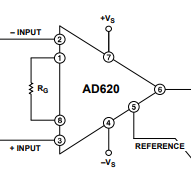
\includegraphics[width=0.4\textwidth]{pictures/hardware/Analog_Interface_board/AD620A.PNG}
	\caption{Instrumentation amplifier AD620A}
	\label{fig:AD620A}
\end{figure} 

The input reference to the \textit{AD620A} has to be very exact. Small differences can cause great inaccuracies in the current measuring. Therefore a voltage reference is used to keep a stable voltage at $0.5V$. The used voltage reference used is a \textit{LM385Z-1.2} in conjunction with a voltage divider of resistors $R1 = 1k\ohm$, $R2 = 1k\ohm$, $R3 = 470\ohm$ yields a constant voltage of

\begin{equation}
	V = V_{ref} \cdot \frac{R1}{R1+R2+R3} = 0.5V
\end{equation}

where 

\begin{equation}
V_{ref} = 1.235V
\end{equation}

A buffer is added to give a low impedance signal to the \textit{AD620A}.

At the input of the instrumentation amplifier a resistor is placed at both the inverting and the non-inverting input to reduce current. Using the \textit{AD620A} is also advantageous for its high CMRR (Common-mode Rejection ratio) that helps with cancelling out noise present on both input pins with the same waveform. It can also use the $\pm15V$ dual supply present on the board.

\subsubsection{Torque pedal measurement}
The output of the torque pedal connects to the same ADC as one of the current channels, hence it also has to be in the range of $0-1V$. The pedal is basically a $7.5k\ohm$ potmeter, so the idea is to parallel it with the lower resistor of a voltage divider to get about $1V$ at full range. Using $V_{ref_3} = 3.3V$ as excitation for the divider and $R1 = R2 = 10K\ohm$, the following equation is true at full throttle: 

\begin{equation}
	V = V_{ref_3} \cdot \frac{R_{pot} \cdot R15}{R_{pot} \cdot R15 + R14} = 0.99V
\end{equation}

When the pedal is not pressed at all, the $0\ohm$ of the potmeter shunts the supply to the ground.

\begin{figure}[H]
\centering
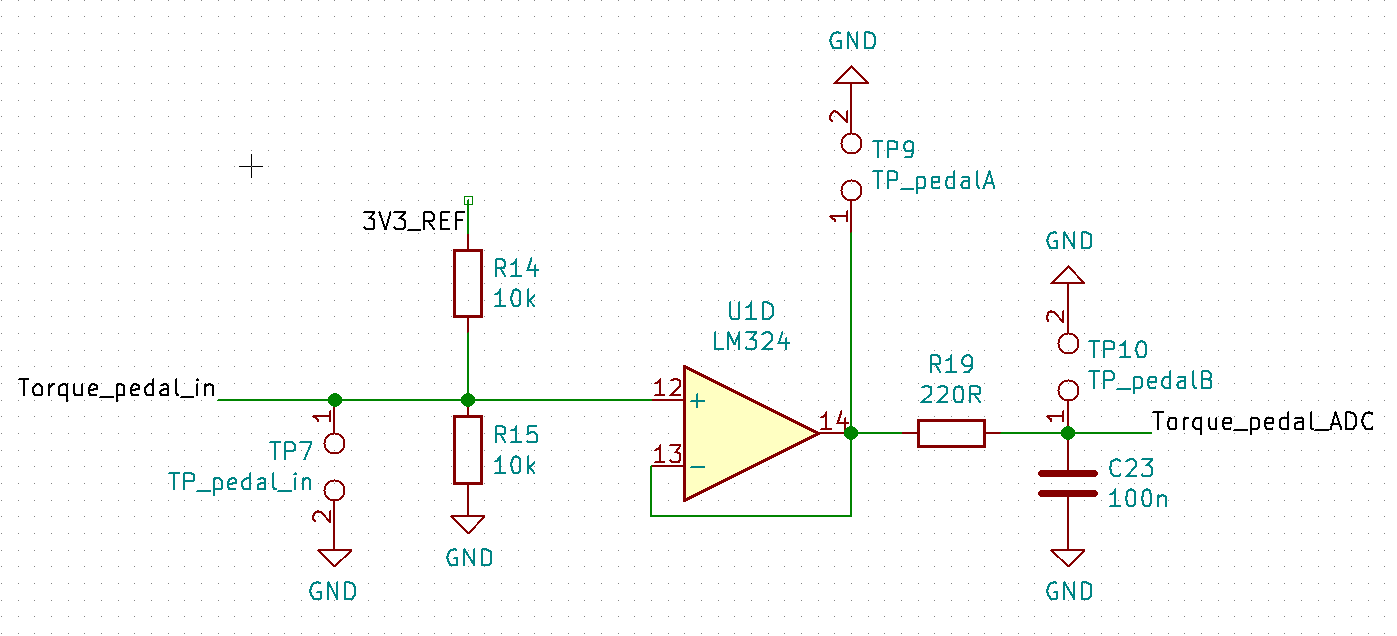
\includegraphics[width=1\linewidth]{pictures/hardware/Analog_Interface_board/torque_pedal_divider.png}
\caption{Torque pedal reading circuit}
\label{fig:torque_pedal_divider}
\end{figure}

For this channel, an opamp in voltage follower configuration is sufficient instead of an instrument amplifier, since no offsetting is required.